\documentclass[smaller,handout,table]{beamer}

\usetheme{clecturesty}

\subtitle{Lecture 1 of 5}

\begin{document}

{
\logo{
\includegraphics[width=0.30\textwidth]{imperialblue}}
\begin{frame}
  \titlepage
\end{frame}
}

\section{Introduction}
\subsection{The Course}

\begin{frame}
\frametitle{Introduction to the Course}
This course has been adapted from its previous incarnation, run by Dr Steve Capper.\\
Originally, the course was based on the M3SC course run by Dan Moore.
\begin{block}<+->{Aims of the Course}
\begin{itemize}
\item To introduce C programming from scratch.
\item To provide insight into scientific computing.
\item To write fast, efficient and maybe even multi-threaded code!
\end{itemize}
\end{block}

\begin{block}<+->{Five lectures}
\begin{itemize}
\item Each afternoon will consist of a $\approx 1$ hour lecture
\item A $\approx 1$ hour practical session.
\end{itemize}
\end{block}
\end{frame}

\begin{frame}
\frametitle{Course Content}
\begin{block}<+->{What we'll cover}
\begin{itemize}
\begin{small}
\item Different number types in C (Integers and Floating Point).
\item Operators, operands and their precedence.
\item Conversions and casts.
\item Mathematical and Logical expressions.
\item Statements: if, else, ?, while, do, for, switch$\ldots$
\item Functions.
\item Pointers, arrays and matrices.
\item Characters, strings and interacting with the console.
\item Reading and writing files.
\item Optimisation and Debugging.
\item Scientific C-Libraries and their uses: NAG, GSL, etc.
\item An Introduction to Parallel Computing.
\item C++ and other languages.
\end{small}
\end{itemize}
\end{block}
\end{frame}

\subsection{What is C}
\begin{frame}
\frametitle{A Rough History of C}
\begin{block}<+->{Invented $\approx{1970}$}
By Dennis Ritchie working in Bell Labs USA; to facilitate development of
a portable UNIX.
\end{block}
\begin{block}<+->{C has been standardised}
\begin{itemize}
\item 1989 ANSI standard ratified \emph{ANS X3.159-1989}.
\item 1990 ISO standard \emph{ISO/IEC 9899:1990}. Aka \emph{C90}.
\item 2000 ISO standard \emph{ISO/IEC 9899:1999}. Aka \emph{C99}.
\end{itemize}
\end{block}
\begin{block}<+->{C++ has evolved from C}
Bjarne Stroustrup developed C++ (C with class). Unlike C, C++ is still under
very active development (C++11 being the most recent standard at the time of
writing).
\end{block}
\end{frame}

\begin{frame}
\frametitle{What are C and C++?}
\begin{itemize}
\item C is a cross-platform, compiled, general-purpose language.
\item C++ can loosely be thought of as C's object-oriented big brother.
\end{itemize}
\begin{alertblock}<+->{}
The vast majority of the programs running on your computer (including the operating system kernel), are written in either C or C++.\\
In the case of Windows, another big contender for a lot of the more recent applications is C\# (but it isn't appropriate at kernel-level or for fast number-crunching).
\end{alertblock}
\end{frame}


\begin{frame}
\frametitle{Why Use C? (Over Maple, Matlab$\ldots$ Excel(?!)$\ldots$)}
\begin{block}<+->{Speed}
C programs are compiled to machine code, the resulting routines \emph{can} run several orders of magnitude quicker than their equivalents in interpreted environments.
\end{block}

\begin{block}<+->{Flexibility}
The C language is intrinsically low level, one can manipulate complex data structures with surprisingly little code.
\end{block}

\begin{block}<+->{Portability}
A well written C program can target many different environments (Windows PCs, Linux workstations, Apple Macs, DEC Alphas, Embedded devices$\ldots$).
\end{block}
\end{frame}

\section{Getting Started}
\subsection{Software}
\begin{frame}
\frametitle{Getting Started}
You will need:
\begin{itemize}
\item A C compiler (many different ones to choose from, some are free).
\item Some documentation (such as the lecture notes/exercises from this course,
a good book, online guides).
\item Lots, and lots of time.
\end{itemize}
\end{frame}

\begin{frame}
\frametitle{Commercial C Compilers}
\begin{itemize}
\item {\tt Intel} - for Windows or Linux. Compiles highly optimised code for Intel (and AMD) processors. Free for personal use and academic use by students. Full-academic and commercial licenses obtainable from:
\url{http://www.polyhedron.com}
\item{\tt Microsoft Visual Studio 2010 Professional} - Microsoft's flagship compiler. Ninety day free trial available at:
\url{http://www.microsoft.com/visualstudio/en-us/try}
\end{itemize}
\end{frame}

\begin{frame}
\frametitle{Free C Compilers}
\begin{block}<+->{Linux}
\begin{itemize}
\item {\tt gcc} - The GNU Compiler Collection, C compiler.
\url{http://gcc.gnu.org}.
\end{itemize}
\begin{block}<+->{Windows}
\begin{itemize}
\item {\tt Visual C++ 2010 Express} - Microsoft's free compiler,
\url{http://www.microsoft.com/express/vc/}
\item {\tt MinGW} - Minimalist GNU for Windows,
\url{http://www.mingw.org/}.
\end{itemize}
\end{block}
\end{block}
\end{frame}

\begin{frame}
\frametitle{Integrated Development Environments}
gcc (for Linux or MinGW) is a command line driven compiler; an Integrated Development Environment (IDE) is a graphical application that provides tools to assist with editing, compiling and debugging of code. I'd recommend Visual Studio Professional as an IDE, this can be obtained through DreamSpark if you're eligible. For a non-windows or free alternative, I'd recommend:
\begin{block}{}
\begin{description}
\item[Windows] \texttt{Visual C++ 2010 Express}, the free Microsoft IDE. \url{http://www.microsoft.com/express/vc/}
\item[Windows/Linux/Mac] \texttt{Code::Blocks}, a cross-platform, open source IDE. \url{http://www.codeblocks.org/}
\end{description}
\end{block}
\end{frame}

\subsection{Books}
\begin{frame}
\frametitle{Books for C}
\begin{block}<+->{Kernighan and Ritchie (K\&R2)}
\begin{columns}
\begin{column}{8cm}
\emph{The C Programming Language}, {\emph Second Edition},
Prentice Hall. This is a fantastically structured reference book, it is written by the authors of C and is \textbf{the} C reference!
\end{column}
\begin{column}{1.5cm}
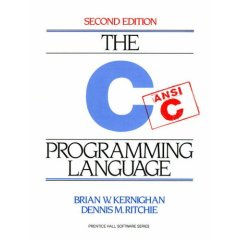
\includegraphics[width=\textwidth]{kandr.png}
\end{column}
\end{columns}
\end{block}

\begin{block}<+->{\emph{Numerical Recipes in C}}
\begin{columns}
\begin{column}{1.5cm}
\includegraphics[width=\textwidth]<2>{nr.png}
\end{column}
\begin{column}{8cm}
By Press, Teukolsky, Vetterling \& Flannery, {\emph Second Edition}, CUP.
Full of high quality example scientific C code. A free online edition can be found at:
\url{http://www.nr.com}\\*There is also a C++ edition in paper or online format.
\end{column}
\end{columns}
\end{block}
\end{frame}

\subsection{Building a C Program}
\begin{frame}
\frametitle{Building a C Program}
\begin{itemize}
\item To \emph{build} an executable from source, we carry out the following
three steps:
\begin{columns}
\begin{column}{3.1cm}
\begin{block}<+->{Edit Source}
Use a text editor to create a {\tt .c} file.
\end{block}
\end{column}
\begin{column}{3.8cm}
\begin{block}<+->{Compile}
With a C compiler, this creates \emph{object file(s)}.
\end{block}
\end{column}
\end{columns}
\begin{columns}
\begin{column}{3.8cm}
\begin{block}<+->{Link}
Combine the object files together into an \emph{executable}.
\end{block}
\end{column}
\end{columns}
\vspace{0.2in}
\item<+-> These steps are can be automated by \emph{Integrated Development Environments}
(IDEs).
\end{itemize}
\end{frame}

\section{Writing C}
\subsection{Hello World}
\ifhandout
\begin{frame}[fragile]
\frametitle{The Traditional Way to Start}
\begin{semiverbatim}
\kr\kl\kw{#include} \kt{<stdio.h>}
\kl
\kl\kw{int} main(\kw{void})
\kl\{
\kl   printf(\kt{"Hello World!\\n"});
\kl   \kw{return} 0;
\kl\}
\end{semiverbatim}

\begin{block}{The ``Hello World'' Program}
A traditional first program started by Ritchie. This is one of the smallest possible C programs that demonstrates some functionality (printing to screen).
\end{block}

\begin{block}{Line 1}
A \emph{pre-processor directive} (it begins with a {\tt \#}) advertising extra routines to the compiler.
\end{block}
\end{frame}

\begin{frame}
\begin{block}{Line 2}
An empty line, or equivalently, a line consisting solely of \emph{whitespace}. This is ignored by the compiler but makes the source code more readable.\end{block}

\begin{block}{Line 3}
A \emph{function declaration}, defining our {\tt main} function. The
{\tt main} function is where our program starts and is known as an
\emph{entry point}. Our main function takes \emph{no parameters} (\kw{\tt void}) and \emph{returns} an integer (\kw{\tt int}).
\end{block}

\begin{block}{Line 4}
\emph{Opening brace}, all statements enclosed between the braces {\tt\{}, {\tt\}} belong to the {\tt main} function.
\end{block}

\end{frame}

\begin{frame}
\begin{block}{Line 5}
A \emph{statement}; the \kw{\tt printf} (print formatted) function is called with the argument \kt{\tt "Hello World!$\backslash$n"}. This prints:\\
{\tt Hello World!}\\
to \emph{standard output} (usually a text console).
\end{block}

\begin{block}{Line 6}
A \emph{return statement}, we exit {\tt main} with a return code of 0. The system interprets 0 as ``success''.
\end{block}


\begin{block}{Line 7}
A \emph{closing brace}, everything after this line does not belong to
{\tt main}.
\end{block}

\end{frame}

\else
\begin{frame}[fragile]
\frametitle{The Traditional Way to Start}
\begin{semiverbatim}
\alert<2>{\kr\kl\kw{#include} \kt{<stdio.h>}}
\alert<3>{\kl}
\alert<4>{\kl\kw{int} main(\kw{void})}
\alert<5>{\kl\{}
\alert<6>{\kl   printf(\kt{"Hello World!\\n"});}
\alert<7>{\kl   \kw{return} 0;}
\alert<8>{\kl\}}
\end{semiverbatim}

\only<1>{\begin{block}{The ``Hello World'' Program}
A traditional first program started by Ritchie. This is one of the smallest possible C programs that demonstrates some functionality (printing to screen).
\end{block}
}

\only<2>{\begin{block}{Line 1}
A \emph{pre-processor directive} (it begins with a {\tt \#}) advertising extra routines to the compiler.
\end{block}}

\only<3>{\begin{block}{Line 2}
An empty line, or equivalently, a line consisting solely of \emph{whitespace}. This is ignored by the compiler but makes the source code more readable.\end{block}
}

\only<4>{\begin{block}{Line 3}
A \emph{function declaration}, defining our {\tt main} function. The
{\tt main} function is where our program starts and is known as an
\emph{entry point}. Our main function takes \emph{no parameters} (\kw{\tt void}) and \emph{returns} an integer (\kw{\tt int}).
\end{block}
}

\only<5>{\begin{block}{Line 4}
\emph{Opening brace}, all statements enclosed between the braces {\tt\{}, {\tt\}} belong to the {\tt main} function.
\end{block}
}

\only<6>{\begin{block}{Line 5}
A \emph{statement}; the \kw{\tt printf} (print formatted) function is called with the argument \kt{\tt "Hello World!$\backslash$n"}. This prints:\\
{\tt Hello World!}\\
to \emph{standard output} (usually a text console).
\end{block}
}

\only<7>{\begin{block}{Line 6}
A \emph{return statement}, we exit {\tt main} with a return code of 0. The system interprets 0 as ``success''.
\end{block}
}

\only<8>{\begin{block}{Line 7}
A \emph{closing brace}, everything after this line does not belong to
{\tt main}.
\end{block}
}

\vspace{10in}
%\vfill
\end{frame}
\fi

\subsection{C Syntax}
\ifhandout
\begin{frame}[fragile]
\frametitle {Another C Program - What does this do?}
\begin{semiverbatim}
\kr\kl\kw{#include} \kt{<stdio.h>}
\kl
\kl\kw{int} main(\kw{void})
\kl\{
\kl   \kw{int} low=-40, high=140, step=5, f, c;
\kl   c = low;
\kl   \kw{while} (c <= high)
\kl   \{
\kl      f = 32+9*c/5;
\kl      printf(\kt{"%6d \\t %6d\\n"}, c, f);
\kl      c = c + step;
\kl   \}
\kl   \kw{return} 0;
\kl\}
\end{semiverbatim}

\end{frame}

\begin{frame}
\begin{block}{Lines 1, 2, 3 \& 4}
Identical meaning as in the previous program.
\end{block}

\begin{block}{Line 5}
\emph{Local variable declarations}; the integers {\tt low}, {\tt high},
{\tt step}, {\tt f} and {\tt c} are declared. These are local to {\tt main}.
The variables {\tt low}, {\tt high} and {\tt step} are \emph{initialised}
with the values; whilst {\tt f} and {\tt c} are \emph{undefined}.
\end{block}
 
\begin{block}{Line 6}
The local variable {\tt c} is \emph{assigned} the value of
{\tt low}.
\end{block}

\begin{block}{Lines 7, 8 \& 12}
A \emph{while} loop is defined. For as long as the variable {\tt c} is less than or equal to {\tt high}, the code between the braces on lines 8 and 12 is executed.
\end{block}

\end{frame}

\begin{frame}
\begin{block}{Line 9}
The local variable {\tt f} is assigned a value from the integer arithmetic expression involving {\tt c}.
\end{block}

\begin{block}{Line 10}
The variables {\tt c} and {\tt f} are printed to standard out, each six characters
wide, separated by a tab and two spaces.
\end{block}

\begin{block}{Line 11}
The local variable {\tt c} is incremented by {\tt step}.
\end{block}

\begin{block}{Lines 13 \& 14}
Have an identical meaning as in the last program.
\end{block}

\end{frame}

\else
\begin{frame}[fragile]
\frametitle {Another C Program - What does this do?}
\begin{semiverbatim}
\only<1-4>{\alert<2>{\kr\kl\kw{#include} \kt{<stdio.h>}}
\alert<2>{\kl}
\alert<2>{\kl\kw{int} main(\kw{void})}
\alert<2>{\kl\{}
\alert<3>{\kl   \kw{int} low=-40, high=140, step=5, f, c;}
\alert<4>{\kl   c = low;}}
\only<1,5->{\alert<5>{\krr{7}\kl   \kw{while} (c <= high)}
\alert<5>{\kl   \{}
\alert<6>{\kl      f = 32+9*c/5;}
\alert<7>{\kl      printf(\kt{"%6d \\t %6d\\n"}, c, f);}
\alert<8>{\kl      c = c + step;}
\alert<5>{\kl   \}}
\alert<9>{\kl   \kw{return} 0;}
\alert<9>{\kl\}}}
\end{semiverbatim}

\only<2>{\begin{block}{Lines 1, 2, 3 \& 4}
Identical meaning as in the previous program.
\end{block}}
 
\only<3>{\begin{block}{Line 5}
\emph{Local variable declarations}; the integers {\tt low}, {\tt high},
{\tt step}, {\tt f} and {\tt c} are declared. These are local to {\tt main}.
The variables {\tt low}, {\tt high} and {\tt step} are \emph{initialised}
with the values; whilst {\tt f} and {\tt c} are \emph{undefined}.
\end{block}}
 
\only<4>{\begin{block}{Line 6}
The local variable {\tt c} is \emph{assigned} the value of
{\tt low}.
\end{block}}

\only<5>{\begin{block}{Lines 7, 8 \& 12}
A \emph{while} loop is defined. For as long as the variable {\tt c} is less than or equal to {\tt high}, the code between the braces on lines 8 and 12 is executed.
\end{block}}

\only<6>{\begin{block}{Line 9}
The local variable {\tt f} is assigned a value from the integer arithmetic expression involving {\tt c}.
\end{block}}

\only<7>{\begin{block}{Line 10}
The variables {\tt c} and {\tt f} are printed to standard out, each six characters
wide, separated by a tab and two spaces.
\end{block}}

\only<8>{\begin{block}{Line 11}
The local variable {\tt c} is incremented by {\tt step}.
\end{block}}

\only<9>{\begin{block}{Lines 13 \& 14}
Have an identical meaning as in the last program.
\end{block}}
\vspace{10in}
\end{frame}
\fi

\begin{frame}
\frametitle{Commenting C Programs}
A comment is text in the source file that gets ignored by the compiler. This is useful for providing human-readable notes about what the code is doing, or removing lines of code temporarily. There are two ways of commenting files in C:

\begin{block}<+->{Traditional Way}
Anything between {\tt /*} and {\tt */} is a comment, i.e.\\
{\tt \kc{/* This function is used to compute the} }\\
{\tt \kc{roots of a quadratic equation */}}
\end{block}

\begin{block}<+->{C++ Style}
These are single line only, anything after {\tt //} is a comment, i.e.\\
{\tt \kw{int} c = 3; \kc{// set c to 3}}

\begin{alertblock}{}
Technically, C++ style comments aren't in the C standard. (But they are
ubiquitous to C code anyway).
\end{alertblock}
\end{block}

\end{frame}

\begin{frame}
\frametitle{Variable Names}
\begin{block}<+->{From K\&R}
``... Is a sequence of letters and digits. The first character must be a letter; the underscore \_ counts as a letter. Upper and lower case letters are different.''
\end{block}

\begin{alertblock}<+->{What to Avoid$\ldots$}
\begin{itemize}
\item Punctuation or any other symbols are not allowed in variable names.
\item The modern C standard discourages the use of an underscore as the first character of a variable name.
\end{itemize}
\end{alertblock}
\end{frame}

\subsection{Preprocessor Directives}
\begin{frame}
\frametitle{Preprocessor Directives}
\begin{itemize}
\item<+-> One example is:
\begin{center}
\tt \kw{\#include} \kt{<stdio.h>}
\end{center}
Which tells the compiler to search \kt{\tt <stdio.h>} for functions.
\item<+-> Another example is:
\begin{center}
\tt \kw{\#define} MAXSIZE 1024
\end{center}
This replaces all occurrences of {\tt MAXSIZE} with {\tt 1024}.
\begin{itemize}
\item Define statements can be named in a similar way to variables, but
\item It is convention to use upper case for \kw{\tt \#define} statements.
\end{itemize}
\item<+-> Or even simpler:
\begin{center}
\tt \kw{\#define} NDEBUG
\end{center}
Meaning {\tt NDEBUG} is defined. This will be expanded later on.
\end{itemize}
\end{frame}


\section{Numbers}
\subsection{Number Types}
\begin{frame}[fragile]
\frametitle{Numbers in C}
There are two types of number in C:
\begin{block}<2->{Integers}
Integers are a type of number that can only hold one of a finite range of whole number values.
\end{block}
\begin{block}<3->{Floating Point Numbers}
Floating point numbers are more flexible and provide an approximation to real numbers. They store a representation of a number in a form with a similar concept to scientific notation.
\end{block}
\end{frame}

\subsection{Integers}
\begin{frame}{Integers}
Integer types in C can be thought of as rings of different sizes (i.e. hours on a clock face). They hold one of the range of integers in the ring and once the highest value in the ring is reached the next incremental value will be the lowest value in that ring.
\begin{itemize}
\item As integers lose all fractional data, multiplication is not always the inverse of division.
\item Products higher than the size of the ring will wrap to the smallest value in the ring; division is not necessarily the inverse of multiplication.
\end{itemize}

\begin{block}{Integer Types}
\kw{{\tt short}, {\tt unsigned short}, {\tt int}, {\tt unsigned int}, {\tt long}, {\tt unsigned long}, {\tt long long}, {\tt unsigned long long}}
\end{block}
\end{frame}


\begin{frame}
\frametitle{Integer Types - For a 32 bit program}
\resizebox{\textwidth}{!}{
\rowcolors[]{1}{blue!20}{blue!10}
\begin{tabular}{r !{\vrule} r l}
\bf Type&\bf Min&\bf Max\\
\hline
short&-32768&32767\\
unsigned short&0&65535\\
int&-2147483648&2147483647\\
unsigned int&0&4294967295\\
long&-2147483648&2147483647\\
unsigned long&0&4294967295\\
long long&-9223372036854775808&9223372036854775807\\
unsigned long long&0&18446744073709551615
\end{tabular}}
\vspace{2ex}\\
For example, here are two bit patterns for \kw{\tt short}:
\begin{center}
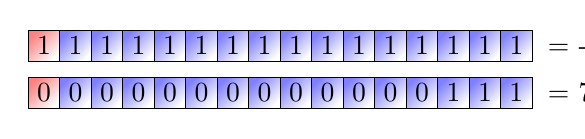
\begin{tikzpicture}[]
\shadedraw [top color=red!50,shading angle=45] (0,0) rectangle +(0.4,0.4);
\node at (0.2,0.2) {0};
\foreach \x in {0.4, 0.8, ..., 6.4}
   \shadedraw [top color=blue!50,shading angle=45] (\x,0) rectangle +(0.4,0.4);
\foreach \x in {0.6, 1.0, ..., 5.0}
   \node at (\x, 0.2){0};
\foreach \x in {5.4, 5.8, 6.2}
   \node at (\x, 0.2){1};   
\node at (6.6, 0.2){\rlap{= 7}};

\shadedraw [top color=red!50, shading angle=45] (0,0.6) rectangle +(0.4,0.4);
\foreach \x in {0.4, 0.8, ..., 6.4}
   \shadedraw [top color=blue!50, shading angle=45] (\x,0.6) rectangle +(0.4,0.4);
\foreach \x in {0.2, 0.6, ..., 6.6}
   \node at (\x, 0.8){1};
\node at (6.6, 0.8){\rlap{= -1}};
\end{tikzpicture}
\end{center}
(for more information see \kt{\tt <limits.h>})
\end{frame}


\begin{frame}
\frametitle{Integer Types}
\begin{itemize}
\item Two main subtypes \emph{signed} and \emph{unsigned}. Signed types use a sign bit.
\item For signed types we, usually, have:
\begin{itemize}
\item minimum value: $-2^{\textrm{size}-1}$
\item maximum value: $2^{\textrm{size}-1}-1$
\end{itemize}
\item For unsigned types we have:
\begin{itemize}
\item minimum value: $0$
\item maximum value: $2^{\textrm{size}}-1$
\end{itemize}
\item \kw{\tt short} is often used to conserve memory.
\item \kw{\tt int} represents the \emph{native} CPU integer type so is used for speed. (If in doubt use \kw{\tt int}).
\item \kw{\tt long} and \kw{\tt long long} are used to maintain accuracy.
\end{itemize}
\end{frame}

\begin{frame}
\frametitle{Integer Arithmetic}

\begin{block}{Base Operators}
The four usual operators are defined $+$, $-$, {\tt *} and $/$.
\end{block}

\begin{block}{Ring arithmetic}
Division is not always the reverse of multiplication:\\
{\tt 1/2=0,  0*2=0.}\\
Also, any result of a computation must lie within the ring, any number outside the range of the current data type will ``wrap'' around. (i.e. 11am + 3 hours gives 2pm).
\end{block}

\begin{block}{Modulo Operator}
The remainder operator {\tt\%} is unique to integer types, it acts as expected:
{\tt7\%2 = 1}.
\end{block}
\end{frame}

\subsection{Floating Point}
\begin{frame}{Floats}
These are much more flexible numbers, but still \emph{NOT} the same as $\mathbb{R}$.
\begin{itemize}
\item Because of the way the number is stored, even fairly simple-looking base-10 numbers ($0.1, 0.2, 0.3\ldots$) are only stored as an approximation.
\item Because numbers are kept as approximations: associativity and commutativity don't always apply and multiplicative inverses don't always exist.
\item The way in which the numbers are stored can result in a loss of the least significant parts of numbers. This causes problems when adding/subtracting big and small numbers together.
\item Programming floats well for numerical problems, especially with large/small numbers, is an art form!
\end{itemize}

\begin{block}{Float Types}
\kw{{\tt float}, {\tt double}, {\tt long double}}
\end{block}
\end{frame}

\begin{frame}
\frametitle{Floating Point Numbers (IEEE 754 Standard)}
On my machine, a \kw{\tt float} (single precision) looks like:\\
\begin{center}
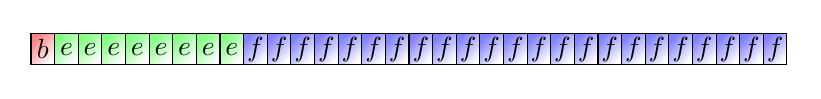
\begin{tikzpicture}[]
\shadedraw [top color=red!50,shading angle=45] (0,0) rectangle +(0.3,0.4);
\node at (0.15,0.2) {$b$};
\foreach \x in {0.3, 0.6, ..., 2.7}
   \shadedraw [top color=green!50,shading angle=45] (\x,0) rectangle +(0.3,0.4);

\foreach \x in {0.45, 0.75, ..., 2.85}
   \node at (\x,0.2) {$e$};
   
\foreach \x in {2.7, 3.0, ..., 9.6}
   \shadedraw [top color=blue!50,shading angle=45] (\x,0) rectangle +(0.3,0.4);
   
\foreach \x in {2.85, 3.15, ..., 9.45}   
   \node at (\x,0.2) {$f$};
\end{tikzpicture}
\end{center}
It consists of three parts, the \textcolor{red}{\emph{sign bit}$(b)$}, the \textcolor{green}{\emph{biased exponent}$(e)$} and the \textcolor{blue}{\emph{fraction}$(f)$}.
We break down a number $x$:
$$x^{\textrm{float}} = \textcolor{red}{(-1)^b} \times 
\textcolor{green}{2^{e-127}} \times \textcolor{blue}{\left(1+f\times2^{-23}\right)},
\begin{array}{c}
0 < e < 255\\0 \leq f \leq 2^{23}-1
\end{array},$$
We have four special numbers, {\tt -Inf} ($-\infty$), {\tt Inf} ($\infty$), {\tt NaN} (Not a Number) and zero.

For \kw{\tt double} (double precision) we have:
$$x^{\textrm{double}} = (-1)^b\times 2^{e-1023}\times\left(1+f\times2^{-52}\right),
\begin{array}{c}
0 < e < 2047\\0 \leq f \leq 2^{52}-1
\end{array}.$$
\end{frame}

\begin{frame}
\frametitle{Floating Point}
\begin{block}{Base Operators}
As with integers, we have $+$, $-$, {\tt *} and $/$.
\end{block}

\begin{block}{Floating point code}
\begin{itemize}
\item It looks like integer code but with a decimal point suffix.
\item Scientific notation is achieved with {\tt e}:\\
{\tt \kw{double} speedofLight = 2.997e8;} ($2.997 \times 10^8$)
\end{itemize}
\end{block}

\begin{block}{Float Arithmetic}
\begin{itemize}
\item Division is not always the reverse of multiplication.
\item Operators may not be commutative!
$$ A + B + C \neq A + C + B \qquad \mathrm{(sometimes)}$$
\end{itemize}
\end{block}
\end{frame}

\subsection{Mathematical Functions}
\begin{frame}
\frametitle{More Mathematical Functions in \kt{\tt <math.h>}}
\begin{itemize}
\item Maths functions come with the \emph{ANSI Standard C Library}, which contains many maths functions. To use them we need a:
{\tt \kw{\#include} \kt{<math.h>}}
\item Here some example functions:
\begin{tabular}{l l l l}
\tt sin(x)&\tt asin(x) & \tt sinh(x) & \tt exp(x)\\
\tt cos(x)&\tt acos(x) & \tt cosh(x) & \tt log(x)\\
\tt tan(x)&\tt atan(x) & \tt tanh(x) & \tt log10(x)\\
\tt sqrt(x)&\tt atan2(x,y)&\tt pow(x,y) & \tt fabs(x)
\end{tabular}\\
\vspace{1ex}
(all the trigonometric functions use radians!)
\end{itemize}
\end{frame}

\begin{frame}
\frametitle{The {\tt pow(x, y)} function (declared in \kt{\tt <math.h>})}
\begin{block}{Exponentiation}
There is no exponentiation operator (e.g. $\wedge$, {\tt **}) in C. Instead we have the following:
$$x^y = \mathrm{\tt pow(x,y)}$$
This assumes $x$ and $y$ are of type \kw{\tt double}.
\end{block}

\begin{alertblock}{Beware}
The {\tt pow} function is often implemented as:
\begin{center}{\tt exp(y*ln(x))}\end{center}
For whole integer powers (i.e. $x^2$), one should perform the multiplication explicitly ({\tt x*x}).
\end{alertblock}
\end{frame}


\section{Control Flow Statements}
\subsection{Logical Expressions}
\begin{frame}
\frametitle{Simple Logical Expressions}
\texttt{\krr{7}\kl   \kw{while} (c <= high)}\\ 
\begin{itemize}
\item Are used to carry out branches ({\tt \kw{if}} statement) and loops (such as {\tt \kw{for}}, and {\tt \kw{while}}).
\item Evaluate to either \emph{true} (non-zero \kw{\tt int}) or \emph{false} (zero).
\end{itemize}

\begin{block}{Logical Operators}
\begin{center}
\begin{tabular}{l c l l}
\tt x &\tt>&\tt  y& is {\tt x} greater than {\tt y}?\\
\tt x &\tt>=&\tt y& is {\tt x} greater than or equal to {\tt y}?\\
\tt x &\tt<&\tt  y& is {\tt x} less than {\tt y}?\\
\tt x &\tt<=&\tt y& is {\tt x} less than or equal to {\tt y}?\\
\alert{\tt x }&\tt\alert{==}&\alert{\tt y}&\alert{is {\tt x} equal to {\tt y}?}\\
\tt x &\tt!=&\tt y& is {\tt x} different to {\tt y}?
\end{tabular}
\end{center}
\end{block}
\end{frame}

\begin{frame}{Using == Safely}
\begin{block}<+->{}
The danger of the easily-made typo:\\
\texttt{\kw{if} (x \alert{=} 3) \{\emph{Statement};\}}\\
is it will \textbf{always} return true and execute the statement, it will also overwrite \texttt{x} with \texttt{3}. This is not only undesirable as it is will not be testing the desired expression, but it is valid code so will not always throw an error - making debugging very tricky.
\end{block}
\begin{block}<+->{A Preventative Measure}
If the variables \texttt{x} and \texttt{3} were to be swapped, such as:\\
\texttt{\kw{if} (3 \alert{==} x) \{\emph{Statement};\}}\\
Then if \texttt{=} was used rather than \texttt{==} it would cause an error as a value cannot be assigned to 3, but it keeps the expression logically equivalent. Getting into the habit of using the variables this way round can save hours of debugging!
\end{block}
\end{frame}

\begin{frame}
\frametitle{Compound Logical Expressions}
We can create compound logical expressions using the following operators:
\begin{itemize}
 \item {\tt ||} is a \emph{logical or}. {\tt le1 || le2} returns false if both {\tt le1} and {\tt le2} are false and true otherwise.
 \item {\tt \&\&} is a \emph{logical and}. {\tt le1 \&\& le2} returns true if and only if both {\tt le1} and {\tt le2} are true.
 \item {\tt !} is a \emph{logical not}. {\tt !le1} returns the opposite of {\tt le1}.
\end{itemize}
Here are two identical examples:
\begin{itemize}
\item \tt (x < 100) \&\& (x\%2 == 0)\\
\item \tt (x < 100) \&\& !(x\%2)
\end{itemize}
\end{frame}

\subsection{Control Statements}
\begin{frame}[fragile]
\frametitle{Flow Control - {\tt if}}
Executes block(s) of code depending on the evaluation of a logical expression.
\begin{block}{Simple {\tt if}}
\begin{center}{\tt \kw{if} (}\emph{logical expression}{\tt ) \{}\emph{statements}{\tt ;\}}\end{center}
\end{block}

\begin{block}{{\tt if}, {\tt else if}, {\tt else}}
\begin{semiverbatim}
   \kw{if} (\emph{logical expression})
      \{\emph{statements};\}
   \kw{else if} (\emph{logical expression})
      \{\emph{statements};\}
   \kw{else if} (\emph{logical expression})
      \{\emph{statements};\}
   \kw{else}
      \{\emph{statements};\}
\end{semiverbatim}
\end{block}
\end{frame}

\begin{frame}[fragile]
\frametitle{Flow Control - {\tt while}}
A \kw{\tt while} loop is used to repeatedly execute code as long as a logical expression is true.

\begin{block}{Structure}
\begin{semiverbatim}
   \kw{while} (\emph{logical expression})
      \{ \emph{statements} ;\}
\end{semiverbatim}
\end{block}
\begin{itemize}
\item If \emph{logical expression} is false, then the \emph{statements} are never executed.
\end{itemize}
\end{frame}

\begin{frame}[fragile]
\frametitle{Flow Control - {\tt do \{\} while ()}}
We place the \emph{logical expression} after the \emph{statements} giving us:
\begin{block}{Structure}
\begin{semiverbatim}
   \kw{do} \{\emph{statements};\}
   \kw{while} (\emph{logical expression})
\end{semiverbatim}
\end{block}
\begin{itemize}
\item The \emph{statements} are executed at least once.
\end{itemize}
\begin{exampleblock}{{\tt do while} or {\tt while}?}
Generally I prefer {\tt \kw{while}} over {\tt \kw{do while}}, as it forces me to initialise variables properly.
\end{exampleblock}
\end{frame}

\begin{frame}[fragile]
\frametitle{Flow Control - {\tt for} loop}
\begin{block}{}
\begin{semiverbatim}
   \kw{for} ( \emph{start expression} ;
         \emph{logical expression} ;
         \emph{step expression})
         \{ \emph{statements} ;\}
\end{semiverbatim}
\end{block}
\begin{itemize}
\item Print out ten numbers:
\begin{semiverbatim}
   \tt\kw{for} (x=0; x < 10; x = x + 1)
      printf(\kt{"x = %d\\n"}, x);
\end{semiverbatim}
\item Keep looping indefinitely (printing out dots)
\begin{semiverbatim}
   \kw{for} (;;) printf(\kt{"."});
\end{semiverbatim}
\end{itemize}
\end{frame}

\begin{frame}[fragile]
\frametitle{Flow Control - \tt switch - case}
We can selectively execute code based on a value, using the following:
\begin{block}{}
\begin{semiverbatim}
   \kw{switch} (\emph{integer\_statement}) \{
   \kw{case} \emph{integer\_value1}: \emph{statements1}; \kw{break};
   \kw{case} \emph{integer\_value2}: \emph{statements2}; \kw{break};
   \kw{case} \emph{integer\_value3}:
   \kw{case} \emph{integer\_value4}: \emph{statements3}; \kw{break};   
   \kw{default}: \emph{statements4}; \kw{break};\}
\end{semiverbatim}
\end{block}
\begin{itemize}
\item Execution starts at either one of the \kw{\tt case}'s or at \kw{\tt default}.
\item Execution stops at the end {\tt\}} or at \kw{\tt break}.
\item \kw{\tt case}, \kw{\tt default} and \kw{\tt break} are optional.
\end{itemize}
\end{frame}

\begin{frame}{Some Loop Control Features}
Execution of code inside a loop (\kw{\tt do}, \kw{\tt while}, \kw{\tt for})
can be manipulated by the following statements.
\begin{block}{\tt break;}
Break out of the current loop. Any statements in the loop following the \kw{\tt break} are ignored and the loop condition automatically evaluates to false, ending the loop.
\end{block}
\begin{block}{\tt continue;}
Jump to the end of the current loop (effectively ignoring everything below the \kw{\tt continue} statement. Whether or not the loop continues executing depends on the loop condition.
\end{block}
\end{frame}

\section{Interacting with the Console}
\subsection{printf}
\begin{frame}
\frametitle{{\tt printf} - declared in \kt{\tt <stdio.h>}}
As seen in the examples, the {\tt printf} function can be used to print out variables. The function \emph{prototype} takes the form:
\begin{center}
{\tt \alert<4>{\kw{int}} printf(\alert<2>{\kw{char} * formatString}, \alert<3>{...})}
\end{center}
\begin{block}<2>{{\tt formatString}}
The first argument of {\tt printf} is the \emph{format string}, this specifies how many variables need printing out, how they are to be printed, and in what order.
\end{block}
\begin{block}<3>{{\tt ...}}
This is C shorthand for \emph{variable number of arguments}.
\end{block}

\begin{block}<4>{Return value: {\tt int}}
{\tt printf} returns the number of characters printed.
\end{block}
\end{frame}

\begin{frame}
\frametitle{{\tt printf} - declared in \kt{\tt <stdio.h>}}
We call {\tt printf} as follows:
\begin{center}
\tt printf(formatString, var1, var2, $\ldots$, varN);
\end{center}
where,
\begin{block}<+->{\tt formatString}
The format string tells {\tt printf} how many variables need printing. A format string can contain \emph{format specifiers}, these tell {\tt printf} exactly how to print out each variable, some examples:
\begin{tabular}{l l}
\tt\kt{"\%6d"} & print out an integer (6 characters wide).\\
\tt\kt{"\%g"} & print out a floating point number.
\end{tabular}
\end{block}
\begin{block}<+->{\tt var1, ...}
{\tt printf} accepts a variable list of arguments, which can be of different type. Care must be taken to match {\tt formatString} with the variables.
\end{block}
\end{frame}

\begin{frame}
\frametitle{Special Characters}
\begin{itemize}
\item The backslash {\tt $\backslash$} character in C has a special meaning, it is known as the \emph{escape character}.
\item We combine the escape character with other characters, to form an \emph{escape sequence}, here are some examples:
\begin{center}
\begin{tabular}{l r}
\begin{tabular}{r l}
{\tt $\backslash$n} & New line\\
{\tt $\backslash$t} & Tab\\
{\tt $\backslash$b} & Backspace\\
{\tt $\backslash$r} & Carriage return\\
{\tt $\backslash$a} & Bell
\end{tabular}&
\begin{tabular}{r l}
{\tt $\backslash$f} & Form feed (new page)\\
{\tt $\backslash\backslash$} & $\backslash$\\
{\tt $\backslash$"} & "\\
{\tt $\backslash$'} & '
\end{tabular}
\end{tabular}
\end{center}
\end{itemize}
\end{frame}

\subsection{scanf}
\begin{frame}{{\tt scanf()} - Reading Data from Standard Input}
\begin{block}<+->{}
For two variables {\tt A} and {\tt B}, both of type \kw{\tt double}, we use:
\begin{center}
\tt scanf(\kt{"\%lf \%lf"}, \&A, \&B);
\end{center}
\begin{itemize}
\item where the {\tt\%} represent \emph{format specifiers}
\end{itemize}
\end{block}
\begin{block}<+->{Format Specifiers}
Consist of a {\tt\%}, a numerical width specification and a field code:
\resizebox{\textwidth}{!}{
\begin{tabular}{c c}
\begin{tabular}{l l}
\tt d& \kw{\tt int}\\
\tt u& \kw{\tt unsigned int}\\
\tt f& \kw{\tt float} (fixed form)\\
\tt e& \kw{\tt float} (exponential form)
\end{tabular}&
\begin{tabular}{l l}
\tt g & \kw{\tt float} (general form)\\
\tt lf & \kw{\tt double} (fixed form)\\
\tt le & \kw{\tt double} (exponential form)\\
\tt lg & \kw{\tt double} (general form)
\end{tabular}
\end{tabular}}
\begin{itemize}
\item and the {\tt\&} represents the \emph{address} of the variable in memory. This is known as a \emph{pointer reference operator}.
\end{itemize}
\end{block}
\end{frame}

\begin{frame}
\frametitle{Why the {\tt \&A} in {\tt scanf()}?}
\begin{itemize}
\item Functions in C can return only one value.
\item Sometimes we want more than one value to change.
\item If we tell {\tt scanf} \emph{where} the variables are in memory,
{\tt scanf} can change them itself.
\end{itemize}

\begin{alertblock}{}
The ability to manipulate memory directly is what makes C so powerful
(and potentially dangerous).
\end{alertblock}
\end{frame}

\subsection{Touching on Pointers}
\begin{frame}[fragile]
\frametitle{Pointers}
A \emph{pointer} is a variable that stores a memory location, they are declared as follows:
\begin{center}
\tt \kw{double} * ptrA;
\end{center}

\begin{block}<+->{{\tt \&} - Pointer reference operator}
Returns the memory address (pointer to) of a variable.
\begin{semiverbatim}
   ptrA = \&A;   \kc{// ptrA points to A}
\end{semiverbatim}
\end{block}

\begin{block}<+->{{\tt *} - Pointer de-reference operator}
Converts a memory address to a variable:
\begin{semiverbatim}
   * ptrA  = 1.234;      \kc{// A is now 1.234}
\end{semiverbatim}
\end{block}
\end{frame}

\subsection{Summary}
\begin{frame}{Summary}
\begin{list}{$\bullet$}{}
\item C is a cross-platform, compiled language which can produce results much quicker than other methods/languages.
\item We use an IDE to write source, compile, link and debug our C programs.
\item The basic structure of a C program has been demonstrated.
\item There are two categories of number in C: integers and floating point numbers.
\item We have seen how logic and statements can control the flow of a program.
\item \texttt{printf} and \texttt{scanf} will write and read from the console respectively.
\end{list}
\end{frame}

\end{document}
